% This is samplepaper.tex, a sample chapter demonstrating the
% LLNCS macro package for Springer Computer Science proceedings;
% Version 2.20 of 2017/10/04
%
\documentclass[runningheads]{llncs}
%
\usepackage{graphicx}
% Used for displaying a sample figure. If possible, figure files should
% be included in EPS format.
%
% If you use the hyperref package, please uncomment the following line
% to display URLs in blue roman font according to Springer's eBook style:
% \renewcommand\UrlFont{\color{blue}\rmfamily}

\begin{document}
%
\title{Voting on Blockchain}
%
%\titlerunning{Abbreviated paper title}
% If the paper title is too long for the running head, you can set
% an abbreviated paper title here
%
\author{Stanisław Barański}
%
\authorrunning{F. Author et al.}
% First names are abbreviated in the running head.
% If there are more than two authors, 'et al.' is used.
%
\institute{Faculty of Electronics, Telecommunications and Informatics\\
Gdansk University of Technology\\
Gdansk, Poland\\
\email{s160518@student.pg.edu.gda.pl}}
%
\maketitle              % typeset the header of the contribution
%
\begin{abstract}
Blockchain as a technology provides two major properties that are highly desirable in applications like election voting. Those properties are immutability which ensures that no one can modify the data once wrote into a blockchain, there might be concerns if this property is truly desirable for everyone, but I assume this system is designed for healthy subjects. Another property is transparency that allows everyone to validates the election correctness and calculate results on its own. In consequences, one can distrust authorities, while trust voting results.

\keywords{Blockchain \and Tokenization \and Voting}
\end{abstract}
%
%
%
\section{State of the art}
Breaking the Encryption Scheme of the Moscow Internet Voting
System ~\cite{ref_moscow_voting}

\section{Introduction}
Blockchain initially introduced by Satoshi Nakamoto in Bitcoin Whitepaper offered one simple application, i.e. ledger for transferring Bitcoin cryptocurrency. 5 years later Vitalik Buterin proposed generalization to this concept by allowing to process not only transactions but also so-called smart contracts which are in fact scripts run on Ethereum platform. Those “scripts” are executed and validated by all Ethereum nodes and use blockchain as persistent storage. This innovation allowed to create domain-specific behavior on top of Ethereum blockchain, leveraging already existing infrastructure.

\subsection{Tokenization}
Currently, the most popular application of smart contracts is token issuance. Those tokens can represent any arbitrary asset either in the virtual or physical world. One can create tokens for funding his startup; hence token represent company shares. This pattern is called ICO (Initial Coin Offering) or STO (Security Token Offering), alluding to IPO (Initial Public Offering). Another one can issue tokens backed by a physical asset like national currency; bypassing slow and expensive international transfers and taxes from exchanging cryptocurrencies with national currencies. This pattern is called Stable Coin. There are many other token applications particularly vote as a token used here in this survey.

\subsection{Stellar platform}
Ethereum provides high flexibility, mainly because of its fully-fledged smart contracts ecosystem, particularly it’s Turing-complete Solidity language. Stellar on the other hand is a blockchain platform specializing just in one application that is asset tokenization. Thus becoming easier, cheaper and faster than general-purpose Ethereum smart contracts. Here I will try to fit this simple election system into Stellar functionality boundaries.

\section{System proposition}
The goal of the system is to provide the highest level of transparency while keeping sensitive data private. Additionally, it should be illegal to issue more than one vote token to one elector. Hence there should be a way of identifying and authorizing voters. I decided to use a government authorized polish system
“Profil Zaufany” as an identity provider, with the assumption that every eligible voter is registered there. The total number of votes tokens should be limited to the total number of eligible voters. I assume that this number is publicly available on the day of the election. In consequence, everyone can verify that there were no more token issued. Vote token exchanging is permitted intentionally and treated as a feature. It’s no different from the traditional election system where some people delegate their vote decision to one family member who tells them what should they vote on. In this system, it’s possible to send the token and let the receiver to perform vote on thy behalf. This decision possibly allows unhealthy vote trading, so this feature can be easily prohibited by disabling manual path described in the following chapters. Stellar is capable of limiting users who are eligible to receive tokens, but I can not see any benefits from using it in proposed system, where user authentication is done by external service (Profil Zaufany), and authorization is done by our backend, which verifies if user is eligible for token issuance.

\subsection{Architecture}
\begin{figure}
\begin{verbatim}
                         +---------------+
       +----------------+ Client Webapp +--------+
       |                +--------+------+        |
       |                         |               |
+------v----------+              |               |
| Identity        |              |            +--+---------+   +-v-------+
| Provider        |              |            | Stellar    +---> Stellar |
| (Profil Zaufany)|              |            | Horizon API|   | Network |
+------+----------+              |            +--+---------+   +-^-------+
       |            +------------v-----------+   |
       |            | Issuance/Authorization |   |
       +------------+        Server          +---+
                    |                        |
                    +------------------------+
\end{verbatim}
\caption{Stelar based architecture}
\label{fig:ascii-box}
\end{figure}

Ideally, the system should only consist of a client webpage that allows users to interact with the Stellar network, getting rid of the centralized identity provider and issuance/authorization server. Unfortunately proposed system requires a central authorization server for vote token issuance, thus becoming a single point
of failure. This flaw has been addressed at the end of this survey. There are also many proposals on how to achieve identification in the blockchain ecosystem, but I won’t use it in this survey.

\subsection{Authorization}
To protect from double token issuance, the proposed system links each token issuance transaction with a user identifier e.g. national identification number. Link is achieved by attaching HMAC of user identifiers in the transaction MEMO field. Thus all information required to perform authorization is contained in the blockchain itself. In consequence, such a system becomes more transparent. We use HMAC of user identifiers to prevent private data exposure, while still allowing to perform authorization check on a public blockchain. The user is eligible to issue token only if his user identifier HMAC is not present in any issuance transaction made from the distribution account.

\subsection{Vote Token}
We assume that the number of eligible voters is public information. Hence becoming the value of a maximum number of tokens in this election. After asset creation, issuing accounts have to lockout from creating a new asset, so all participants can be sure that no more tokens are ever created. Additionally, it should be impossible to perform vote, after the end of the election. Unfortunately Stellar doesn’t have such feature build-in, although it can be done by blocking all new token issuance on issuance/authorization server, and by revoking all accounts that received token. This would require setting AUTHORIZATION REVOCABLE flag on issuing account.
Assets in stellar blockchain, are divisible to 7 decimal points. This is an unwanted feature since we don’t want to allow users to vote by just one-tenth of their vote. To prevent it, we will treat 1 vote token as the smallest indivisible amount possible in XDR which is 1 scaled down by a factor of 10,000,000 (this format allows to represent decimal numbers in 7 digit precision, without introduction floating-point arithmetics and it’s innate errors).

\subsection{Token distribution}
Each user who authenticates itself by Profil Zaufany and authorizes by our issuance/authorization server will be able to issue 1 voting token (seen by the user as 0.0000001). One can do with this token whatever he wants, ideally votes for one of the eligible parties, but nothing prevents him from transferring this token to any other account, such as a family member. Since it already happens in the current traditional voting system, it should not be considered as a system flaw, rather as a feature.

\subsection{Voting Paths}
Our system allows two paths of voting: simplified and manual. In manual path, the user already possesses a stellar account and wants to take control of the whole process, which involves creating trustline to distribution account and issuing vote token. Simplified path create a new keypair on the frontend side, not revealing the private key to the backend. Client prepare one ACID transaction that includes five operations:
1. Fund newly created account with the minimum required amount of lumens to process next operations. 1 XLM (cryptocurrency used in the stellar blockchain) for minimum account balance, 0.5 XLM for creating a trustline.
2. Create trustline to vote token asset issuer.
3. Send 1 vote token from distribution account to newly created account.
4. Send 1 vote token from newly created account to one of the chosen parties.
5. Distrust from vote token asset issuer in order to merge account.
6. Merge newly created account to distribution account, bringing back
remained XLM.
The prepared transaction is then signed by a newly created account, send to the issuance/authorization server, which performs validation, sign and send it back to the client webapp. Now both issuance/authorization server and the voter can publish the transaction to the stellar network. The user of such path is completely abstracted from technology used underneath, while still leveraging all blockchain benefits. The simplified path could be enhanced by allowing the user to reveal his keypair, hence allowing him to send his vote token to another user, instead of voting on their own, same as on manual path. But just for sake of the proposed system, two separate paths are available.

\subsection{Transaction Fees}
Let’s evaluate the proposed system in the context of transaction fees. To do this we can estimate how much would cost the 2019 Polish parliamentary election, handled by the proposed system. We already know that 18 470 710 people participated in such an election. Each operation on stellar network costs 0.00001XLM. Manual path uses 1 operation (on the issuer side), whereas simplified path uses six operations. Let’s assume that no one possessed a stellar account yet, and everyone chose simplified path. In that case, each vote transaction costs 0.00006XLM. We know that the closing price for one Lumen in the day of the election was 0.229626 PLN. We can easly calculate 18470710 votes * 0.00006 XLM/vote * 0.229626 PLN/XLM = 254.48 PLN. Other operational transactions can be neglected due to very low influence on total sum.

\subsection{Preparation}
To create such an election, we need an issuer and distribution account, a new vote token, and accounts for all registered parties. Creating issuer and distribution account and creating new token is a multi-step process; well described on official stellar documentation Issuing Assets and Custom Assets Each party account is created similar to simplified path described above, but limited to the first two operations. See bootstrap.js for whole flow implementation. Variables that need to be propagated in backend and webpage code are:
• asset name, asset issuer public key
• limit of possible vote tokens (number of eligible voters). • token expiration (end of election).
• distribution account public key.
• list of (party name, party account public key).
In the backend, those environment variables are injected from .env file. In fronted, we could do similar using e.g. Webpack DefinePlugin, but for simplicity, I decided to not use any bundler.
Now the application is ready to be published.

\subsection{Fully Decentralized Blockchain Application}
In the blockchain world in order to ensure absolute trust, everything should be blockchain contained, which is often hard, impractical and/or expensive. For example one could encode all eligible user addresses (or better hash of addresses) in smart contract and then allow redeeming vote token only to addresses which are present in there, very similar to traditional election system where all eligible voters are listed on paper, vote form is issued only if elector is present on such list. While this might work for a small list of addresses, it can become overkill for election when the cost of such a huge smart contract is taken into account. Fortunately, there are already blockchains that allow linking data from outside the blockchain, i.e. ethereum oracle. To ensure immutability and integrity, such data can be hosted on IPFS (Content Addressed Network) where data is identified by its hash example.

\subsection{Demo}
Demo represents the 2019 Polish parliamentary election, but for the sake of simplicity, the number of eligible voters equals 100. The created token is called Vote01122019. The demo can be accessed on https://voting.stasbar.com or locally

\section{Results}
The proposed system prototype satisfies core expectations. Authorities can not falsify election results. There is a limit on how much votes can be issued. Each vote is recorded on Blockchain, and everyone can calculate election results without trusting authorities. What we get is a system where Blockchain is the only subject who needs to be trusted. Both government and electoral can distrust each other, while still perform valid elections (assuming that they trust Blockchain). We confirmed that Blockchain can be used not only for cryptocurrencies but also in assets tokenization and building dapps (decentralized applications). Stellar is just one of many platforms that could be used in such cases, but it turns out that it handles it very well. What makes Stellar one of the best options in this category is transaction fees, were estimated costs of 2019 Polish parliamentary election to 254.48zł. To estimate transaction speed we would need to host a local instance of Stellar Horizon API server to isolate from network latency and possible queueing overhead. Doing it would also allow to accurately measure how the proposed system behaves on heavy overload. It would be interesting to compare such system on different blockchain platforms.

\paragraph{Sample Heading (Fourth Level)}
The contribution should contain no more than four levels of
headings. Table~\ref{tab1} gives a summary of all heading levels.

\begin{table}
\caption{Table captions should be placed above the
tables.}\label{tab1}
\begin{tabular}{|l|l|l|}
\hline
Heading level &  Example & Font size and style\\
\hline
Title (centered) &  {\Large\bfseries Lecture Notes} & 14 point, bold\\
1st-level heading &  {\large\bfseries 1 Introduction} & 12 point, bold\\
2nd-level heading & {\bfseries 2.1 Printing Area} & 10 point, bold\\
3rd-level heading & {\bfseries Run-in Heading in Bold.} Text follows & 10 point, bold\\
4th-level heading & {\itshape Lowest Level Heading.} Text follows & 10 point, italic\\
\hline
\end{tabular}
\end{table}


\noindent Displayed equations are centered and set on a separate
line.
\begin{equation}
x + y = z
\end{equation}
Please try to avoid rasterized images for line-art diagrams and
schemas. Whenever possible, use vector graphics instead (see
Fig.~\ref{fig1}).

\begin{figure}
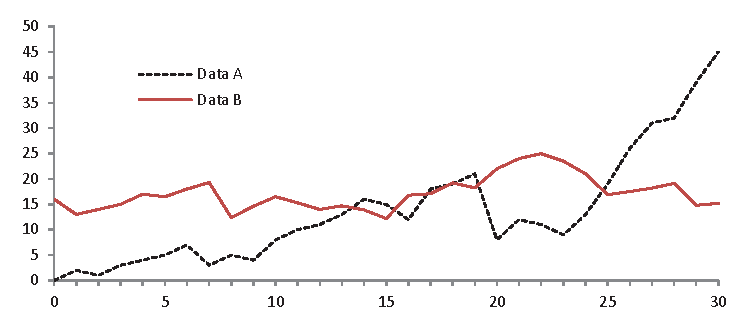
\includegraphics[width=\textwidth]{fig1.eps}
\caption{A figure caption is always placed below the illustration.
Please note that short captions are centered, while long ones are
justified by the macro package automatically.} \label{fig1}
\end{figure}

\begin{theorem}
This is a sample theorem. The run-in heading is set in bold, while
the following text appears in italics. Definitions, lemmas,
propositions, and corollaries are styled the same way.
\end{theorem}
%
% the environments 'definition', 'lemma', 'proposition', 'corollary',
% 'remark', and 'example' are defined in the LLNCS documentclass as well.
%
\begin{proof}
Proofs, examples, and remarks have the initial word in italics,
while the following text appears in normal font.
\end{proof}
For citations of references, we prefer the use of square brackets
and consecutive numbers. Citations using labels or the author/year
convention are also acceptable. The following bibliography provides
a sample reference list with entries for journal
articles~\cite{ref_article1}, an LNCS chapter~\cite{ref_lncs1}, a
book~\cite{ref_book1}, proceedings without editors~\cite{ref_proc1},
and a homepage~\cite{ref_url1}. Multiple citations are grouped
\cite{ref_article1,ref_lncs1,ref_book1},
\cite{ref_article1,ref_book1,ref_proc1,ref_url1}.
%
% ---- Bibliography ----
%
% BibTeX users should specify bibliography style 'splncs04'.
% References will then be sorted and formatted in the correct style.
%
% \bibliographystyle{splncs04}
% \bibliography{mybibliography}
%
\begin{thebibliography}{8}

\bibiterm{ref_moscowvoting}
\bibitem{ref_moscow_voting}
Author, P. Gaudry, Author A. Golovnev: Breaking the Encryption Scheme of the 
Moscow Internet Voting System

\bibiterm{ref_verifiability}
\bibitem{ref_verifiability}
Author, V. Cortier, Author. D. Galindo, Author. R. Kusters, Author. J. Muller, Author. T. Truderung: SoK:
Verifiability Notions for E-Voting Protocols

\bibitem{ref_article1}
Author, F.: Article title. Journal \textbf{2}(5), 99--110 (2016)

\bibitem{ref_lncs1}
Author, F., Author, S.: Title of a proceedings paper. In: Editor,
F., Editor, S. (eds.) CONFERENCE 2016, LNCS, vol. 9999, pp. 1--13.
Springer, Heidelberg (2016). \doi{10.10007/1234567890}

\bibitem{ref_book1}
Author, F., Author, S., Author, T.: Book title. 2nd edn. Publisher,
Location (1999)

\bibitem{ref_proc1}
Author, A.-B.: Contribution title. In: 9th International Proceedings
on Proceedings, pp. 1--2. Publisher, Location (2010)

\bibitem{ref_url1}
LNCS Homepage, \url{http://www.springer.com/lncs}. Last accessed 4
Oct 2017
\end{thebibliography}
\end{document}

